\documentclass[12pt]{article}
\usepackage[english]{babel}
%\usepackage{subcaption}
\usepackage{hyperref}
\usepackage{graphicx}
\usepackage{amsmath}
\graphicspath{{images/}}
\usepackage{geometry}
 \geometry{
 a4paper,
 total={170mm,257mm},
 left=20mm,
 top=20mm,
 }
\begin{document}
\section{Image Classification using Convolutional Neural Network} 
\subsection{Introduction}
In this project, we are given a dataset containing the images of dogs and cats. The images in the dataset are divided for training and testing. The goal of this project is to create a convolutional neural network which can learn to recognize an image and say whether it is dog or a cat. This report contains a detailed description of the pipeline and the details of the neural net used. 

\subsection{Software Used:}
\begin{enumerate}
\item Python 3
\item Google Colab
\item Jupyter Notebook
\end{enumerate}

\subsection{Packages Used:}
\begin{enumerate}
\item Pytorch
\item torchvision
\end{enumerate}

\subsection{Implementation using Google Colab:}
We using Google Colab to train our neural net using the GPU available present in it. We uploaded the dataset to google drive and linked the Google Colab and drive. Hence, we were able to access the dataset present in Google drive directly from Google Colab.

\subsection{Pipeline Employed}
\begin{enumerate}
\item \textbf{Data Preparation:} The input dataset provided contains of train and test folder. The cat and dog images in train folder were mixed. So, we prepared a separate folders for both cat and dog images in train folder. 

\item \textbf{Pre-Processing the dataset:}Before training the neural net, we converted the image into gray. This is because color of the image did not give any feature. With or without color, the number of features remained the same. Moreover, in color images there were three channels which increased number of computations when convolution operation is performed in neural net. After converting the images to gray we stored it in a .npy file in order to access it further during training.

\item \textbf{Neural Net Architecture:}
This is the neural network we used for training and testing the model.
\newpage
\begin{figure}[h]
    \centering
    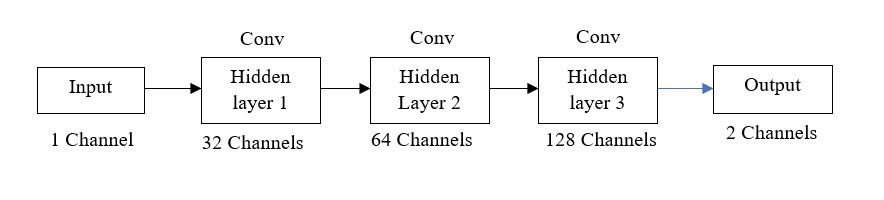
\includegraphics[width=16cm]{nn}
    \caption{Neural Network}
    \label{fig:Neural Network}
\end{figure}
The neural network consists of three hidden layers. The first layer consists of 32 channels. The second layer consists of 64 channels. The third layer consists of 128 channels. The neural network takes input 

\item \textbf{Training the Neural Net:}
After creating the neural net, we need to pass the data for neural net to train. We now load the stored .npy file while contains the training images of dogs and cats of the training data stored in numpy array. In addition to this, the accuracy and loss obtained in each EPOCH is stored to plot.

\item \textbf{Testing the Neural Net:}
The testing is performed on the neural net in the similar way as training. The labelled data which is not considered for training is considered for testing and accuracy and loss are calculated for varying number of EPOCH. 

\subsection{Improving Accuracy of the neural network:}
Initially, by considering number of EPOCH as 2, the accuracy was about 75. Improvement in the accuracy was obtained by increasing the number of EPOCH  to 20. The final batch size considered after tweaking was 100. 

\subsection{Outputs:}
Following are the graphs obtained for accuracy and loss with respect to number of EPOCH both for training and testing data. From the output graphs, it can be inferred that the accuracy of the neural net increases and loss decreases with the increases in number of EPOCHS.\\
\textbf{Training Results:}
\begin{figure}[h]
    \centering
    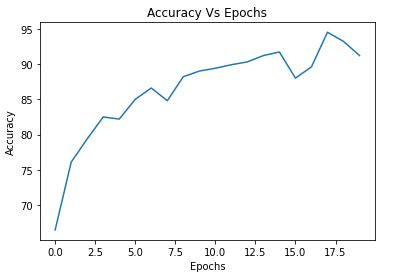
\includegraphics[width=9.5cm]{accuracy_train}
    \caption{Accuracy Results}
    \label{fig:Accuracy Results}
\end{figure}
\newpage
\begin{figure}[h]
    \centering
    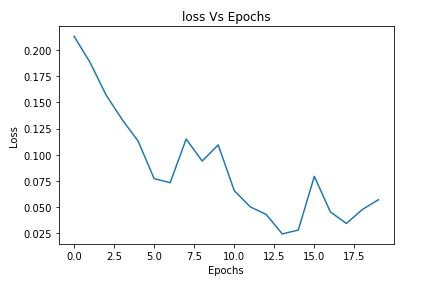
\includegraphics[width=9.5cm]{loss_train}
    \caption{Loss Results}
    \label{fig:Loss Results}
\end{figure}
\end{enumerate}
\section{Team Members:}
1. Eashwar Sathyamurthy
2. Akwasi A Obeng
3. Achal P Vyas
\end{document}